\chapter{Stand der Forschung}

Im folgenden Kapitel wird ein grundlegendes Verständnis für die Funktionsweise von Strukturbatterien vermittelt. Außerdem werden die Besonderheiten im Vergleich zu konventionellen Batterien und faserverstärkten Verbundwerkstoffen erläutert. Dazu werden die wichtigsten Eigenschaften und deren Ermittlungsverfahren dargestellt sowie die Rolle der einzelnen Komponenten im Zusammenhang mit der Materialauswahl näher erklärt. Anschließend werden aktuelle Entwicklungsansätze diskutiert und abschließend die ungelösten Herausforderungen mit den aktuellen Methoden näher analysiert.

\section{Funktionsweise der Strukturbatterie} Strukturbatterien sind Batterien, die mechanisch belastbar sind und damit auch zur strukturellen Integrität beitragen können.
Batterien erlauben es, temporär Energie zu speichern, indem Ladungsträger reversibel in einem Hostmaterial eingelagert werden. Solche Zellen werden daher auch ''Shuttle-Clock''~\cite{Ohzuku1993}-, ''Rocking-Chair''~\cite{Tarascon1993}- oder ''Swing''~\cite{Bittihn1993}-Zellen genannt. Der Einlagerungsprozess selbst wird meist als ''Interkalation'' bezeichnet~\cite{Eichinger1976}. Durch den Einlagerungsprozess nehmen die beiden Hostmaterialien aktiv am Ladungsaustausch teil, daher auch der Name ''Aktivmaterial'', siehe Bild~\ref{fig:battery_function}. Häufig ist das Aktivmaterial für die Anode Graphit und für die Kathode ein Metalloxid (\ce{MO_2}).
\begin{figure}[ht]
	%\raggedleft
		%\def\svgwidth{\columnwidth}
        \center
	\includegraphics[width=\textwidth, angle=0]{battery_function.pdf}
		\caption{\label{fig:battery_function}Die Energiespeicherfunktion einer Batterie wird maßgeblich durch den skalenübergreifenen Ein- und Auslagerungsprozess der Ladungsträger realisiert.}
\end{figure}
Beim Entladen der Batteriezelle wandern die Ladungsträger von der Anode zur Kathode. An beiden Elektroden kommt es zum Ladungsaustausch, der mittels Redox-Gleichungen beschrieben werden kann~\cite{Goodenough2013}: 
\begin{align}
	\ce{C_6 + x Li^+ + x e^- &<=> Li_xC_6}\\ 
	\ce{LiMO_2 - x Li^+ - x e^- &<=> Li_{1-x}MO_2} 
\end{align} 
Der Einlagerungsprozess erlaubt im Vergleich zur reinen elektrostatischen Speicherung, wie etwa bei Kondensatoren, eine signifikant höhere Beladungsdichte an Ladungsträgern, wodurch größere Energiemengen gespeichert werden können~\cite{Newman2021}.

Entscheidend für die Funktion der Batterie ist hierbei, dass der Transport der Ionen durch den Elektrolyten und den Separator erfolgt. Die Elektronen können jedoch nur entlang des Stromkollektors geleitet werden und müssen daher einen „Umweg“ außerhalb der Zelle machen~\cite{Plett2015}, siehe Bild~\ref{fig:battery_function}. Die Bewegung der Elektronen ist dabei im Vergleich zum Ionentransport deutlich schneller, weshalb die Ent- und Beladungsgeschwindigkeit einzig von der Ionenmobilität limitiert wird~\cite{Plett2024}.

Im Falle großer Ströme, wie etwa bei einem Kurzschluss, finden viele Ladungsumwandlungsreaktionen gleichzeitig statt. Die dabei entstehende Wärme kann zum Versagen oder Brennen der Zelle führen. Mögliche Ursachen für Kurzschlüsse sind Herstellungsfehler, Dendritwachstum und mechanische Belastungen, bei denen die Elektroden durch Versagen des Separators in direkten Kontakt kommen, wie etwa bei Penetration oder Biegung~\cite{Beard2019}.

Darüber hinaus führt die mit den mechanischen Belastungen einhergehende Rissbildung zu einer Erhöhung des inneren elektrischen Widerstandes, was zu einem Verlust an Speichereffizienz führt und daher vermieden werden soll~\cite{Plett2024}. Bei konventionellen Batterien kommen daher spezielle Umhausungen zum Einsatz, die eine Belastung der Batterien verhindern sollen~\cite{Beard2019}. Diese bringen allerdings einen signifikanten Anteil an zusätzlicher Masse hinzu und sind aufgrund ihrer Größe meist schwerer in Hoststrukturen zu integrieren~\cite{Asp2021}. Um diesen Nachteilen zu begegnen, versuchen Strukturbatterien durch die Integration geeigneter Materialien die mechanische Belastungsfähigkeit zu verbessern~\cite{Carlstedt2018}. Zur Steigerung der Multifunktionalität neuer Strukturbatterien ist daher neben einem umfangreichen Verständnis der wichtigsten Eigenschaften auch ein Überblick über mögliche Materialkandidaten aus bestehenden Untersuchungen zu konventionellen Batterien sowie dem Leichtbaubereich notwendig~\cite{Asp2019}.


\section{\label{sec:Ermittlungsverfahren}Stand der Forschung zu wichtigsten Ermittlungsverfahren}

Das Interesse an Strukturbatterien kommt aus zwei verschiedenen Fachbereichen: der konventionellen Batterieforschung und dem integrativen Leichtbau. Beide Bereiche betrachten diese Technologie im Kontext unterschiedlicher Referenzsysteme. Dies führt dazu, dass die Strukturbatterie sowohl mit den aktuellsten Hochleistungsbatterien, wenn es die elektrochemsiche Leistungsfähigkeit geht, als auch mit Karbonfasern im Kontext von mechansicher Steifigkeit und Festigkeit verglichen wird~\cite{O’Brien2011,Snyder2015}. Daraus leitet sich die Bedingung ab, dass jede Strukturbatterie so zu charakterisieren ist, dass ein Vergleich beider Seiten möglich ist. Darüber hinaus stellen perspektivische Anwendungen, wie der Automobilbereich~\cite{Martins2021,Pistoia2010}, die Luftfahrt~\cite{Ishfaq2022} und wachsende ökologische Bedenken~\cite{EU2023}, ein breites Spektrum an Anforderungen, die den Charakterisierungsaufwand weiter erhöhen. 
Der große Anteil an nicht-standardisierten Ermittlungsverfahren stellt dabei zusätzlich eine ernstzunehmende Herausforderung dar~\cite{Greenhalgh2023,Zschiebsch2024}. In diesem Kapitel soll daher ein Überblick über die wichtigsten Größen und in der Forschung benutzten Messmethoden zur Bestimmung dieser gegeben werden.
Brennbarkeit~\cite{Shirshova2021,Shirshova2024}, \ce{CO2}-Produktion und Recyclingfähigkeit~\cite{Heyadati2024} sind zwar von wachsender Bedeutung, ihre Bestimmungsmaßnahmen sind jedoch sehr wenig normiert und spielen in der aktuellen Strukturbatterieforschung eine vergleichsweise untergeordnete Rolle. Sie werden daher hier nicht ausführlicher diskutiert.




%\subsection{Interkalation}
\subsection{Ladungszustand}
Ein wesentliches Merkmal von Batterien ist die Einlagerung von Ionen in das Hostmaterial (Interkalation). Je nach Hostmaterial steht dabei eine bestimmte Menge an Einlagerungsplätzen zur Verfügung. Der Ladungszustand (\textit{engl.} state of charge, SOC) beschreibt den Anteil der besetzten Plätze an den insgesamt verfügbaren Plätzen~\cite{Plett2015}.

Das bedeutet, dass, wenn alle Plätze belegt sind, der SOC gleich 1 bzw. 100~\% ist, und wenn alle Ionen das Hostmaterial verlassen haben, also keiner der Plätze belegt ist, der SOC einen Wert von 0~\% hat. Alternativ wird der Beladungszustand auch durch die stöchiometrische Größe $x$ angegeben, die besonders häufig im Kontext der Beschreibung von Zwischenzuständen (z.B. \ce{Li_xMn2O4} oder \ce{Li_{1-x}C}) benutzt wird~\cite{Newman2021}. Der SOC hat maßgeblichen Einfluss auf das chemische Potenzial (siehe Bild~\ref{fig:battery_voltage}), die Volumenausdehnung (siehe Tabelle~\ref{tab:volume_change}) und die Diffusionsgeschwindigkeiten~\cite{Plett2024}. Der SOC kann jedoch nicht direkt gemessen werden und wird stattdessen über die Elektrodenspannung ermittelt~\cite{Newman2021}.

\begin{table}[ht]
    \centering
    \caption{\label{tab:volume_change}Volumenänderungen bo der Lithiierung für gängige Aktivmaterialien.}
    \begin{tabular}[t]{lccc}
        \toprule
        Material& Volumenänderung $\Delta$V/V\textsubscript{0}&Verlauf&Referenz\\
        \midrule
        Graphit & +10\% - +13\% & nicht-linear & \cite{Qi2010,Woodford2012}\\
        NMC111 &-2,4\%&nicht-linear& \cite{Yabuuchi2005}\\
        NMC422 &+2,4\%&nicht-linear& \cite{Ma2007}\\
        LCO &-1,9\% & linear & \cite{Reimers1992}\\
        NCA &-1,6\% & nicht-linear& \cite{Itou2005}\\
        LFP &+6,5\% & linear & \cite{Padhi1997}\\
        LMO &+6,6\% & linear & \cite{Christensen2006}\\
        \bottomrule
    \end{tabular}
\end{table}

\subsection{Elektrische Spannung}

Die elektrische Spannung ist neben dem Strom, der direkt mit der Bewegung der Ladungsträger verbunden ist, eine der wichtigsten Größen zur Beschreibung des Zustandes in einer Batteriezelle~\cite{Beard2019}. 

\begin{figure}[ht]
    \center
		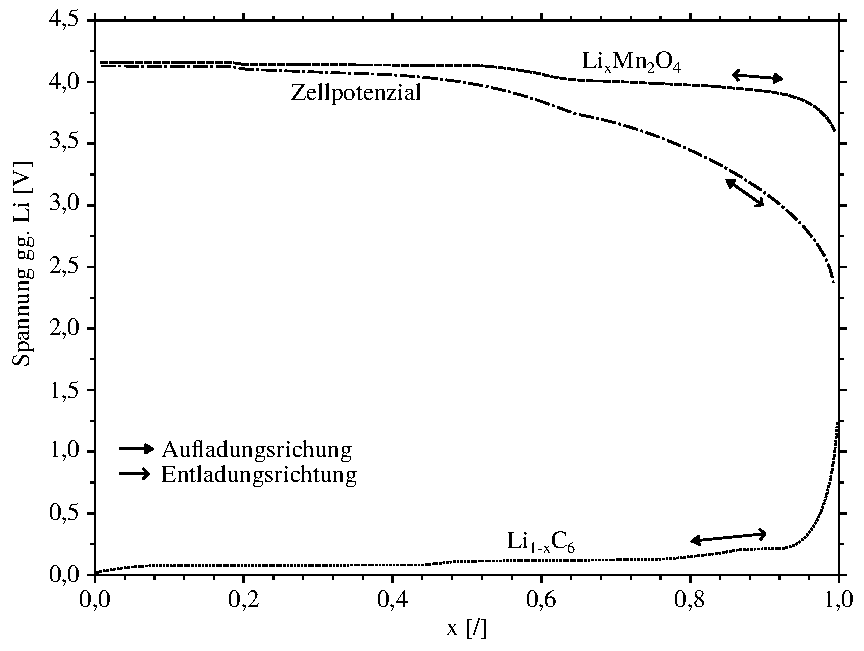
\includegraphics[width=\textwidth, angle=0]{uocp.pdf}
		\caption{\label{fig:battery_voltage}Spannung über den stöchiometrischen Anteil der beladung einer Lithiumionenbatterie, sowie die Anteile der negativen (Graphit) und positiven (Manganoxid) Elektrode (angelehnt an~\cite{Newman2021}).}
\end{figure}

Im Kontext der Elektrochemie ist die elektrische Spannung ein Maß für das elektrochemische Potenzial einer Elektrode. Ein Potenzial kann jedoch nur durch den Vergleich zu einem Referenzpotenzial, das dann oft als ''Nullpotenzial'' bezeichnet wird, gemessen werden. In der Batterieforschung wird hierbei häufig die Referenzspannung gegen reines Lithium gemessen~\cite{Newman2021}. Entscheidend ist hierbei, dass diese Referenzspannung bei einer Elektrode nicht konstant ist, da sich durch das Ein- und Auslagern das chemische Potenzial verändert. Der resultierende Funktionsverlauf ist abhängig von der chemischen Struktur und kann damit Aufschlüsse auf das Einlagerungsverhalten und damit verbundene Phasenumwandlungen geben~\cite{Plett2015}, siehe Bild~\ref{fig:battery_voltage}.

Damit Batterien sich nicht selbst entladen, wenn ein Verbraucher angeschlossen ist, ist es wichtig, dass die Zellspannung, auch als nominale Spannung bezeichnet, mit zunehmender Entladung stetig sinkt~\cite{Newman2021}, siehe Bild~\ref{fig:battery_voltage}. Der reversible Lithiumbeladungsprozess ist dabei stets mit einem abnehmenden Potenzialanstieg an der jeweiligen Elektrode verbunden. Da in einer Batterie durch den Ladungsaustausch immer eine Elektrode beladen wird, während die andere entladen wird, kann der stetige Spannungsabfall während der Entladung sichergestellt werden, wenn die Referenzspannung einer Elektrode immer größer ist als die der anderen~\cite{Plett2024}. Aus dem stetigen Verlauf der Zellspannung leiten sich für die Anwendung weitere wichtige Spannungsgrößen ab: die Abschaltspannung, die die minimal erlaubte Spannung und damit den ''entladenen'' Zustand markiert~\cite{Plett2015}.

Eine weitere wichtige Kenngröße für Batterien ist die Leerlaufspannung, welche gemessen wird, wenn kein Strom zwischen den beiden Elektroden fließt. Daher ist sie von signifikanter Bedeutung für die Beschreibung des Gleichgewichtszustandes innerhalb der Zelle~\cite{Newman2021}.

\subsection{C-Raten}
Die Auflade- oder Entladerate einer Batterie wird oft in sogenannten C-Raten angegeben. Dabei bedeutet 1~C, dass eine vollständig entladene/geladene Batterie in 1~h komplett aufgeladen/entladen wird. Bei einer doppelt so hohen C-Rate wird die Batterie folglich in der Hälfte der Zeit, also 30~min, entladen bzw. aufgeladen. Bei einer halb so hohen Auflade- bzw. Entladerate (0.5C oder C/2) benötigt die Batterie 2~h, um vollständig aufgeladen oder entladen zu werden. Die Wahl der C-Rate ist vor allem bei der Messung der Kapazität von Bedeutung. Verallgemeinert gilt: Je höher die C-Rate, desto geringer ist die gemessene Kapazität. Die Stärke des Kapazitätsabfalls wird durch eine Reihe von Faktoren, wie Übergangsverhalten, Form und Art der chemischen Struktur der Elektrode usw., bestimmt~\cite{Plett2015,Beard2019}.


\subsection{Kapazität}
Die Kapazität einer Elektrode beschreibt, wie viele Ladungsträger eingelagert oder entfernt werden können. Besonders in den ersten Zyklen ist der Unterschied zwischen Auflade- ($\text{C}_{\text{aufl}}$) und Entladekapazität ($\text{C}_{\text{entl}}$) signifikant, weshalb die Kapazität für beide Prozesse getrennt bestimmt wird~\cite{Plett2015}.

Zur Ermittlung der Kapazität wird ein konstanter Auflade- ($\text{I}_\text{C,aufl}$) oder Entladestrom ($\text{I}_\text{C,entl}$) (C-Rate) an eine Zelle aus Elektrode und Referenzelektrode, meist Lithiummetall, angelegt und die Zeit $\Delta \text{T}_\text{aufl}$ gemessen, die für die komplette Auf- bzw. Entladung benötigt wird. Da die Kapazität das zeitliche Integral des Stromes ist, kann die Bestimmung auf die folgenden Formeln vereinfacht werden~\cite{Newman2021}:
\begin{align}
	\text{C}_{\text{aufl}} &= \text{I}_\text{C,aufl} \cdot \Delta \text{T}_\text{aufl}\\
	\text{C}_{\text{entl}} &= \text{I}_\text{C,entl} \cdot \Delta \text{T}_\text{entl}.
\end{align}

%komplett entladen oder in der die Spannung von Abschalt- bzw. Leerspannung $\text{U}_{\text{leer}}$ zur vorher ermittelten maximal Spannung $\text{U}_{\text{voll}}$ benötigt. Die Aufladekapazit stellt dabei das Produkt aus Durch Umkehrung des Prozesses lässt sich die Entladekapazität bestimmen 

Bei der Entwicklung neuer Batteriematerialien wird die Kapazität meist auf die Masse des am Einlagerungsprozess teilnehmenden Materials (Aktivmaterial) normiert. Diese spezifische Kapazität hat dann die Einheit [$\si{\A \hour \per \g}$]. Im Kontext der Batterieentwicklung wird allerdings die Kapazität je Elektrodenfläche [$\si{\A \hour \per \cm\squared}$] häufig angegeben.


\subsection{Columbische Effizienz}
Die coulombsche Effizienz (CE) ist eine der meistbenutzten Metriken, um die interne Reaktion zu bewerten. Die CE des Zyklus \( n \) ist definiert als das Verhältnis der gemessenen Kapazität während des Entladevorgangs \( C_{Dch}(n) \) zur Kapazität des vorherigen Beladungsvorgangs \( C_{Ch}(n) \) \cite{Tornheim2020}.
Die Formel
\begin{equation}
CE = \frac{C_{Dch}(n)}{C_{Ch}(n)}
\end{equation}
gilt dabei für Aufbauten, die in einem Entladenzustand zusammengebaut werden und daher zuerst beladen werden müssen. Zellen, die in einem beladenen Zustand gefertigt werden, wie etwa Lithium-Schwefel-Batterien, beginnen allerdings zuerst mit einem Entladungszyklus. Die korrekte Formel lautet in einem solchen Fall
\begin{equation}
    CE = \frac{C_{Dch}(n+1)}{C_{Ch}(n)}.
\end{equation}

\subsection{Kapaziätserhalt}
Die Kapazitätserhalt (\textit{engl.} Capacity Retention) ist eine wichtige Metrik, um den Anteil an Nebenreaktionen, die zu einem Kapazitätsverlust in Batterien führen, zu bemessen. Sie ist definiert als das Verhältnis von Entladungskapazität des $(n+1)$-ten Zyklus $C_{Dch}(n+1)$ und der des $n$-ten Zyklus $C_{Dch}(n)$:
\begin{equation}
    CE = \frac{C_{Dch}(n+1)}{C_{Dch}(n)}.
\end{equation}
In einigen Fällen wird CR auch im Verhältnis zur initialen Entlade-Kapazität bestimmt, also
\begin{equation}
    CE = \frac{C_{Dch}(n)}{C_{Dch}(1)}.
\end{equation}
Dieser Ansatz ist besonders dann hilfreich, wenn die Langlebigkeit zu bestimmen ist \cite{Tornheim2020}.
Im Gegensatz zu CE ist CR meist relevanter für Hersteller und Endnutzer.

\subsection{Energiedichte}
Die gravimetrische Energiedichte bzw. spezifische Energie bemisst, wie viel Energie pro eingesetzter Masse gespeichert werden kann. Alternativ wird mittels der volumetrischen Energiedichte die Menge an speicherbarer Energie pro Volumen angegeben. Beide Kenngrößen sind wichtige Größen, die bei der Entwicklung neuer Speichertechnologien nach Möglichkeit gesteigert werden sollen~\cite{Plett2015}.

Eine der größten Schwierigkeiten beim Umgang mit angegebenen Energiedichten aus der Literatur besteht in dem Umstand, dass oft bei der Masse oder dem Volumen auf verschiedene Komponenten Bezug genommen wird~\cite{Son2021}. Im Allgemeinen unterscheiden sich die Angaben darin, ob die Werte im Kontext von:
\begin{enumerate}
	\item Materialentwicklung
	\item Elektrodenentwicklung
	\item Zellentwicklung
\end{enumerate}
erhoben wurden, siehe Tabelle~\ref{tab:energy_densities}.
So wird bei der Forschung an neuen Aktivmaterialien die spezifische Energie auf die eingesetzte Masse an Aktivmaterial bezogen. Im Bereich neuer Elektroden wird die Speicherkapazität entweder auf die Elektrodenmasse oder, im Falle einer Oberflächenbeschichtung, meist nur auf die Masse der Beschichtung normiert. In Publikationen zu neuen Zellen gibt es noch mehr Varianten. Je nach Autor finden sich hier Angaben in Referenz zur Masse der gebauten Knopfzelle oder der gebauten Pouchzelle; bei Letzterer gibt es Varianten mit einer einzelnen Zelle oder einer mehrlagigen Ausführung. Außerdem werden in manchen Publikationen die Mantelmaterialien herausgerechnet.
\begin{table}[ht]
    \centering
    \caption{\label{tab:energy_densities}Spezifische Energie und Energiedichte für eine representative \ce{LiCoO2} (LCO) Kathode und eine Grafitanode in verscheidenen Referenzsystemen.\cite{Son2021}}
    \begin{tabular}[t]{lccccc}
    \toprule
    \multirow{2}{*}{}
    &\multirow{1}{*}{Materialevel} % \textsuperscript{*}
    &\multirow{1}{*}{Elektrodenlevel}
    &\multicolumn{2}{c}{Zelllevel}
    \\ \cmidrule{2-5}
    &Aktivmaterial
    &Elektrode
    &Knopfzelle
    &\makecell{Pouchzelle\\(1 Ah)}
    \\
    \midrule
    \makecell{Spezifische Energy\\ $\left[ \si{\watt \hour \per \kg} \right]$} & 627 & 514 & 5 & 260\\
    \makecell{Energiedichte\\ $\left[ \si{\watt \hour \per \liter} \right]$} & 3166 & 1527 & 19 & 414\\
    \bottomrule
    \end{tabular}
    %\noindent{\footnotesize{\textsuperscript{*} Die Abkürzung nicht auffindbar (n.a.) wurde benutzt.}}
\end{table}%
Die beschriebene Uneinheitlichkeit in der Veröffentlichung der Daten ist ein großer Diskussionspunkt in der Batterieforschung und macht es sehr aufwendig, vielversprechende Ansätze zu identifizieren~\cite{Greenhalgh2023, Zschiebsch2024}.

%\subsection{Zyklenverhalten}
\subsection{Steifigkeit und Festigkeit}
\begin{itemize}
	\item finden in der konventionellen Batteriforschung bislang keine Betrachtung
	\item entscheident
	\item SOC hat einfuss auf beides: Festigkeit wird reduziert Steifigkeit wird erhöht
	\item Problem: Ermittlungsverfahren nicht eindeutig (Biegeversuch vs Zugversuch)
\end{itemize}
%\subsection{Mechanische Spannung}
\subsection{Multifunktionale Effizienz}

Die einheitenlose multifunktionale Effizienz ist ein Maß, um zu bewerten, ob ein Vorteil durch den Einsatz von multifunktionalen Lösungen gegenüber einem kombinierten Einsatz von monofunktionalen Komponenten entsteht~\cite{Johannisson2020}.
Der von \textsc{Snyder et al.}~\cite{Snyder2015} im Jahr 2011 veröffentlichte Ansatz beschreibt die multifunktionale Effizienz als Summe der mechanischen und elektrochemischen Effizienz.
\begin{align}
	\eta_{\text{mutli}} &= \eta_{\text{mech}} + \eta_{\text{elchem}}\\
						&= \frac{E}{E_{\text{ref}}} + \frac{\Gamma}{\Gamma_\text{ref}} 
\end{align}
Diese Herangehensweise erlaubt eine vereinfachte Betrachtung der sonst komplexen multidisziplinären Optimierung und ist nach \textsc{Ashby}~\cite{Ashby2000} eine der möglichen Optimierungsstrategien für Materialdesign und -auswahl. In der Strukturbatterieforschung hat sich der Bewertungsansatz mittels multifunktionaler Effizienz weitgehend durchgesetzt~\cite{O’Brien2011,Freund2018}.

Im Kontext von Strukturspeichern wird für die mechanische Effizienz oft das Verhältnis der spezifischen Steifigkeiten, häufig dargestellt durch das Elastizitätsmodul, der multifunktionalen Strukturbatterie und der eines UD-Kohlefasergeleges betrachtet. Ähnlich ergibt sich die elektrochemische Effizienz der Strukturbatterie aus dem Verhältnis der jeweiligen Energiedichten~\cite{Sha2021}. Ein multifunktionaler Effizienzwert größer oder gleich eins bedeutet, dass durch den Einsatz eine Reduktion der Gesamtmasse gegenüber der monofunktionalen Lösung erreicht wird~\cite{Snyder2015}.

\section{Materialkandidaten für Strukutbatterien}

Jedes Material in einer Strukturbatterie erfüllt mehrere Aufgaben gleichzeitig. Dies bedeutet, dass 
die am häufigsten verwendete Untergliederung die Materialien nach ihrer elektrochemischen Rolle einteilt.


\subsection{Anode}
Die Anode sollte ein niedriges elektrochemisches Potenzial und eine schnelle Interkalation für eine möglichst hohe Energiedichte und Leistungsdichte aufweisen. Zusätzlich profitieren Strukturbatterien sehr von Anoden mit hohen Festigkeits- und Steifigkeitswerten.

Die Verwendung von Kohlenstoff in Lithium-Ionen-Batterien wurde erstmals von \textsc{Yoshino} \cite{Yoshino1986} 1986 veröffentlicht, der für diesen Durchbruch 2019 den Nobelpreis erhielt.
Heute ist Kohlenstoff eines der meistbenutzten Materialien in wiederaufladbaren nicht-wässrigen Batterien \cite{Ahmad2021}. Am weitesten verbreitet ist dabei die Kombination von Graphit als Anode und einer Kathode aus Phosphat, welche eine maximale Energiedichte von 200-250~$\si{\watt \hour \per \kg}$ erreicht. 
Es gibt zwei Arten von Kohlenstoff, die in der Lage sind, Ionen einzulagern: geordneter und ungeordneter \cite{Ghosh2024}.

Geordneter Kohlenstoff besteht aus Materialien mit einer weitreichenden Ordnung und hoher Kristallinität. Die Ordnung kann sich dabei auf eine Achse (CNTs), eine Ebene (Graphen) oder den Raum (Graphit) beschränken \cite{Wang2021}.

Graphit hat eine hochkristalline Struktur und besitzt eine weitreichende Ordnung. Die $\text{sp}^\text{2}$-hybridisierten Graphenschichten sind entlang der c-Achse gestapelt und folgen entweder der hexagonalen AB-Sequenz oder der rhomboedrischen ABC-Folge. Die bindenden $\pi$-Orbitale ermöglichen eine gute Leitfähigkeit von $10^3$-$10^4$~$\si{\siemens \per \cm}$ in der Ebenenrichtung. Die Graphenschichten haben einen Abstand von 3,35~$\si{\angstrom}$ entlang der c-Achse und werden nur durch relativ schwache van der Waals-Kräfte (16-17~$\si{\kJ \per \mol}$) zusammengehalten. Der relativ hohe Abstand und die schwachen Bindungskräfte machen es einfach, dass sich kleine Atome wie Lithium oder Kalium zwischen den Ebenen einlagern können \cite{Wang2021}.

Der Interkalationsprozess läuft dabei in vier Stufen ab, was sich im Potenzialverlauf erkennen lässt. Das Lithium-Ion wird dabei zwischen zwei benachbarten Graphenschichten eingelagert, wobei jedes Lithium-Ion den niedrigsten Energiezustand einnimmt, der im Zentrum eines hexagonalen Kohlenstoffrings existiert \cite{Sole2014,Weng2023}. Allerdings können Lithium-Ionen nicht durch die Graphenschichten hindurchtunneln, weshalb die Transportbewegung zwischen den Schichten nur entlang von Gitterdefekten möglich ist \cite{Nishidate2005}. Die Einlagerungsgeschwindigkeit ist dabei nicht konstant und kann während jeder Stufe um teilweise das Tausendfache einbrechen \cite{Levi1997}. Dieses Verhalten kommt nach \textsc{Aurbach et al.} durch die Bildung von Lithium-Clustern zwischen den beiden Graphenschichten zustande, welche die Diffusion weiterer Lithiumionen am Anfang einer neuen Phase verhindern \cite{Markevich2005}. Die maximale Einlagerungsmenge ist mit der $\text{LiC}_\text{6}$-Konfiguration erreicht, bei der zwischen jeder Graphitschicht alle möglichen Plätze belegt wurden. Die Menge an eingelagerten Lithiumionen entspricht dabei einer theoretischen spezifischen Kapazität von 372~$\si{\mA \hour \per \g}$ \cite{Winter1998}. 
Eine weitere wichtige Eigenschaft ist die relativ hohe Dichte von >2~$\si{\g \per \cm \cubed}$, was dabei hilft, möglichst viel Aktivmaterial in kleinem Raum unterzubringen, um kleine Batterien mit einer hohen Energiedichte zu erzeugen.

Seit seiner Entdeckung im Jahr 2004 \cite{Novoselov2004} ist Graphen zunehmend in den Fokus der Batterieforschung geraten. Mit einer theoretischen Kapazität von >1000~$\si{\mA \hour \per \g}$, einer hohen mechanischen Zugfestigkeit von $\approx$130~$\si{\GPa}$ und einer Zugsteifigkeit von $\approx$1~$\si{\tera \Pa}$ stellt es ein ideales Material für den Einsatz in Strukturbatterien dar \cite{Novoselov2012}. Jedoch konnte das Material bisher nur im Labormaßstab und in unzureichenden Mengen synthetisiert werden. Auch ist bisher umstritten, wie die Einlagerung von Lithium bei Graphen genau abläuft, was je nachdem die theoretische Kapazität noch stark nach oben oder unten korrigieren könnte. Bisherige Experimente mit zweilagigem Graphen kommen zu unterschiedlichen Ergebnissen. \textsc{Ji et al.} beobachteten einen Mechanismus, der auf einen ähnlichen Prozess wie bei Graphit schließen lässt, während \textsc{Kühne et al.} sogenannte superdichte Lithiumeinlagerungen zwischen den beiden Graphenschichten gemessen haben wollen. Derzeitig geht die Produktion von Graphen nicht über den Labormaßstab hinaus und bleibt daher für den Einsatz in Strukturbatterien bis auf Weiteres ungeeignet.

CNTs sind geordnete 1D-Kohlenstoffstrukturen, die 1991 von \textsc{Iijima} \cite{Iijima1991} erstmals entdeckt wurden. Diese zylindrischen Formen des Kohlenstoffs haben einen Durchmesser von 1-20~$\si{\nano\metre}$ und meist ein hohes Längen-zu-Durchmesser-Verhältnis, mit der höchsten bisher dokumentierten Länge von 55~$\si{\centi\metre}$ von \textsc{Zhang et al.} \cite{Zhang2013}. CNTs werden meist durch ihre Schichtanzahl in SWCNT und MWCNT unterschieden. Darüber hinaus können SWCNTs, je nach Winkel des graphenähnlichen Gitters im Mantel gegenüber der Zylinderachse, metallische oder halbleiterähnliche Eigenschaften aufweisen. 
SWCNTs und MWCNTs besitzen hohe spezifische Oberflächen (1300~$\si{\m^2\per g}$), eine sehr hohe elektrische Leitfähigkeit (5000~$\si{\siemens \per \cm}$) und eine hohe Ionenleitfähigkeit von (>100000~$\si{\cm \squared \per \V \per \s}$) \cite{Xu2011,Uetani2014,Charlier2007}.

Ungeordneter Kohlenstoff hat keine weitreichende periodische Struktur in Ebenen- oder Stapelrichtung. Er besteht hauptsächlich aus zufällig ausgerichteten sp2-graphitischen Mikrobereichen und Verknüpfungen durch sp3-hybridisierte Kohlenstoffatome in amorphen Gebieten. Der Anteil der sp3-Verknüpfungen bestimmt, ob eine Graphitisierung bei Temperaturen bis zu 3000~$\si{\degreeCelsius}$ möglich ist. Dies führt zu einer Unterscheidung in sogenannten harten oder weichen Kohlenstoff.

Bei weichem oder graphitisierendem Kohlenstoff kann aufgrund der geringen Anzahl von sp3-Verknüpfungen immer noch eine thermisch bedingte Mobilität der Kohlenstoffschichten erfolgen, was bei einer Wärmebehandlung von 1500-3000~$\si{\degreeCelsius}$ unter Sauerstoffausschluss (Pyrolyse) zu einer Umwandlung zu Graphit führt. Ein weitverbreiteter Ansatz zur Herstellung von weichem Kohlenstoff ist die thermische Zersetzung von verschiedenen organischen Precursoren in einer inerten Atmosphäre bei hohen Temperaturen (1000-1700~$\si{\degreeCelsius}$) (Karbonisierung). Besonders geeignet sind hierbei pyrolytische aromatische Verbindungen wie etwa Pech, Benzol, Petrolkoks, Polyvinylacetat und Polyvinylchlorid \cite{Wang2021}. Die Wahl des sogenannten Precursormaterials und der Prozessparameter hat maßgeblichen Einfluss auf die chemische Struktur, die wiederum die Eigenschaften von ungeordnetem Kohlenstoff bestimmt. Besonders entscheidend ist hierbei der Kristallinitätsgrad oder Graphitisierungsgrad, welcher u.a. durch Ramanspektroskopie bestimmt werden kann \cite{Yu2014}. Die mikro-kristallinen Graphitbereiche haben dabei ein ähnliches Einlagerungsverhalten wie Graphit. Die kleinere Menge an graphitischen Strukturen sorgt jedoch dafür, dass die Ionenspeicherkapazität bei einer langsamen Beladung (C/10) von graphitischem Kohlenstoff nur etwa 250~$\si{\mA \hour \per \g}$ (Graphit 372~$\si{\mA \hour \per \g}$) erreicht. Jedoch ist die Einlagerung deutlich schneller, was bei höheren Beladungs- und Entladungstests (10C) zu einer dreimal höheren Kapazität (weicher Kohlenstoff 90~$\si{\mA \hour \per \g}$ und Graphit 25~$\si{\mA \hour \per \g}$) führt \cite{Schroeder2014}. Auch zeigt graphitisierender Kohlenstoff im Gegensatz zu Graphit keine Einbrüche im Diffusionsverhalten, was dafür spricht, dass die Einlagerung stufenlos erfolgt. Allerdings bleiben auch in den weniger geordneten Strukturen mehr Lithiumionen gefangen, weshalb die CE während des ersten Zyklus für weichen Kohlenstoff nur bei etwa 72~\% (Graphit 82~\%) liegt. Jedoch liegt die CE nach dem Prelithierungsprozess auch hier bei über 99~\% \cite{Schroeder2014}.

Harter oder nicht-graphitisierender Kohlenstoff lässt sich selbst bei hohen Karbonisierungstemperaturen (<3000~$\si{\degreeCelsius}$) nicht in Graphit umwandeln. Meist wird dieser aus der Karbonisierung von Precursoren mit wenigen aromatischen Strukturen, wie etwa Zucker, Holzkohle, Cellulose und Kokosnussschalen, gewonnen \cite{Wang2021}. Die komplexeren organischen Strukturen der Precursoren sorgen dafür, dass nach der Karbonisierung eine signifikante Anzahl an kleineren Poren und Rissen in der Mikrostruktur verbleiben, die einen schnellen Zugang zu den Interkalationsbereichen erlauben und für eine hohe aktive Oberfläche sorgen \cite{Liu2019a}. Graphenschichten $\approx$0.4~$\si{\nm}$ in der ungeordneten Mikrostruktur führen zu einer hohen zyklischen Stabilität und einer Kapazitätsretention (CR) von 85~\% nach hunderttausend Zyklen \cite{Cao2014}.

% Eine CAG ist ein hartcarbon?

%Eines der am frühsten und immer noch am weitverbreitesten Aktivematerialien anodenseitig ist Graphit. Zwischen den Graphitschichten können Lithiumionen eingelagert werden. In herkömmlichen monofunktionalen Batterien werden oft dünne Kupferfolien mit einer Graphitpartikelbeschichtung verwendet. Die zusätzliche Additive in der Pulvermischung halten die Partikel zusammen und sorgen für einen geringen Widerstand beim Transport der Elektronen zur Kupferelektrode. Die Bindungen zwischen den Partikeln sind jedoch sehr schwach und tragen nicht zur Steigerung der mechanischen Eigenschaften bei \cite{Chen2024}. Außerdem ~mAh/gsorgt die Ausdehnung infolge von Lithierung mit der Zeit für Risse durch die mit der Zeit der Leitungswiderstand steigt, was einer von vielen beobachten Alterungsmechanismen von Batterien ist \cite{Xiong2020}.

%Die begrenzte Kapazität, langsame Diffusionskinetik, geringe mechanische Eigenschaften, sind einige der Faktoren die Untersuchungen Kohlenstoff-Nanostrukturen und andere Morphologien bewegen.

Kohlenstofffasern sind einer der vielversprechendsten Kandidaten für lasttragende Anoden. Ca. 96~\% aller Fasern weltweit werden aus Polyacrylnitril (PAN) hergestellt, die restlichen werden aus Precursorn wie Pech, Rayon oder Lignin gewonnen \cite{Das2016}. Kohlenstofffasern besitzen im Allgemeinen hohe Festigkeits- und Steifigkeitswerte sowie eine elektrisch gut leitende Oberfläche, die mit 0,2~$\si{\metre\squared\per\g}$ zwar zu klein für Batterieanwendungen ist, jedoch durch verschiedene Oberflächenmodifikationen \cite{Qian2013,Senokos2023} auf über 200~$\si{\metre\squared\per\g}$ gesteigert werden kann \cite{Zenkert2024}. Jedoch haben die Wahl des sogenannten Precursormaterials sowie die Verfahrensparameter während des Spinnens, Stabilisierens und Karbonisierens einen entscheidenden Einfluss auf die Struktur der Faser, was sich wiederum signifikant in den mechanischen, elektrischen und elektrochemischen Eigenschaften bemerkbar macht \cite{Newcomb2015}.

Verallgemeinert lässt sich feststellen, dass ein höherer Anteil an kristallinen Graphitstrukturen in der Faser zu einer höheren Steifigkeit, Festigkeit sowie thermischen und elektrischen Leitfähigkeit führt. Jedoch ist die Kapazität von 150~$\si{\mA\per\g}$ (C/10) bei diesen hochmoduligen Fasern, wie etwa M60J, deutlich geringer als bei Fasern mit niedrigem Kristallinitätsanteil, wie etwa T800 (265~$\si{\mA\per\g}$) und IMS65 (358~$\si{\mA\per\g}$) \cite{Fredi2018}. Man nimmt an, dass die geringere Kapazität durch die relativ großen, sich wie ein Mantel um die Faser ausbildenden Kristallstrukturen und turbostatischen Graphitstrukturen zustande kommt, die einen radialen Ionentransport stark behindern \cite{Zenkert2024}. Bei Fasern mit weniger ausgeprägter Graphitkristallausbildung bieten die zahlreichen Gitterdefekte, ähnlich wie bei ungeordnetem Kohlenstoff, genug Zugang für die Lithiumionen, um sich bei kleineren Beladungsraten vollständig einlagern zu können \cite{Fredi2018}. Dies deckt sich mit Beobachtungen, dass sich Lithium zunächst in den ungeordneten (amorphen) Bereichen einlagert und erst bei höherer Beladung auch die graphitischen Strukturen besetzt werden \cite{Fang2022}. Wie auch bei graphitischen Kohlenstoffen verlieren Kohlenstofffasern einen großen Teil ihrer Ladungsträger während des ersten Zyklus \cite{Jacques2013}. Jedoch bleibt die CE auch nach zehn Zyklen bei über 99,9~\% \cite{Hagberg2016}, was bedeutet, dass der weitere Beladungs- und Entladungsprozess nahezu verlustfrei ist. Allerdings hat die Einlagerung von Ionen auch zur Folge, dass sich die mechanischen Eigenschaften der Fasern ändern. Dabei verdoppelte sich der E-Modul quer zur Faserrichtung im lithierten Zustand und ging während der Delithierung nahezu vollständig auf die Werte im Ursprungszustand zurück. Für das Modul in Faserrichtung konnten dabei allerdings keine Veränderungen gemessen werden \cite{Duan2021}. Weiterführende Zugversuche im lithierten und delithierten Zustand zeigten außerdem, dass die Zugfestigkeit während der Lithierung um 25-30~\% zurückging und selbst nach der Entladung um 5-10~\% geringer war als im ursprünglichen Zustand \cite{Jacques2012}. Versuche mit verschiedenen Lithierungsgraden konnten dabei eine direkte Abhängigkeit zur Zugfestigkeit feststellen \cite{Jacques2014}, was darauf schließen lässt, dass die durch die Einlagerung verursachten Dehnungen im Material maßgeblich den Festigkeitsverlust beeinflussen \cite{Zenkert2024}. Der Festigkeitsverlust im Zusammenhang mit einer multifunktionalen Nutzung muss damit zwar unbedingt berücksichtigt werden, spielt aber besonders bei steifigkeitsgetriebenen Anwendungen eine untergeordnete Rolle, da eine weitere Degradierung der Fasern nicht beobachtet wurde \cite{Zenkert2024}.

\begin{table}[ht]
    \centering
    \caption{Übersicht kohlenstoffbasierter Elektroden.}
    \begin{tabular}[t]{lcccc}
    \toprule
    &\makecell{Kapazität\\$\left[ \si{\mA \hour \per \g} \right]$} % \textsuperscript{*}
    &\makecell{E-Modul\\ $\left[ \si{\GPa} \right]$}
    &\makecell{Zugfestigkeit\\ $\left[ \si{\MPa} \right]$}
    &\makecell{Leitfähigkeit\\ $\left[ \si{\siemens \per \cm} \right]$}
    %&CR [\%] % Capacity Retention
    %&$\text{D}_{\text{Li}}$ %[$\text{cm^2/s}$]
    %&Ref.
    \\
    \midrule
    Graphit
        &356...372 \cite{Winter1998} % Capacity
        &10 \cite{Lin2023} % E-Module
        &31 \cite{Lin2023} % Zugfestigkeit
        &$1000...10000$ \cite{Wang2021} % Leitfähigkeit
        %&98
        %&$10^{-7}-10^{-6}$ ($10^{-11}$\textsuperscript{,K})
        %&\cite{Persson2010,Wang2021,Olutogun2024}\\
        \\
    Graphen
        &770...1115 \cite{Wu2011} % Capacity
        &31 \cite{Lin2023}  % E-Module
        &130 \cite{Lin2023} % Zugfestigkeit
        &2700 \cite{Murata2019} % Leitfähigkeit
        %&100
        %&90
        %&$7 \times 10^{-5}$
        %&\cite{Zhu2014,Wang2017,Kuehne2017}\\
        \\
    CNT
        &400...600 \cite{Boaretto2020}
        &35 \cite{Kim2017}
        &850 \cite{Kim2017}
        &5000 \cite{Charlier2007}
        \\
    %Kohlenstofff Nanoröhren
    %    &1115
    %    &90
    %    &$10^{-14}-10^{-11}$
    %    %&\cite{Maurin1999,Zhao2000,Meunier2002,Shin2002,Nishidate2005,Schauerman2012}\\
    %Harter Kohlenstoff
    %    &200-600 % 0.2C
    %    %802-1063 lade capacitität
    %    % 27.9-47.3 lade/entlade effizienz / Columbic Efficiency
    %    &72-90 % nach 50 Zyklen
    %    &$10^{-9}$-$10^{-8}$
    %    %&\cite{Fujimoto2010,Bridges2012,Yang2012}\\
    %Karbon Aerogel
    %    &349-570,2
    %    &31,9-97%(836.9-570.2)/836.9
    %    &n.a.
    %    %&\cite{Yang2015,Pham2024,Li2022a}\\
    T300
        &130 \cite{Kjell2011}
        &230 \cite{Kjell2011}
        &3530 \cite{Kjell2011}
        &667\cite{Kjell2011}
        %&91
        %&46,5 % (170-91)/170
        %&$10^-12-10^-11$
        %&\cite{Uchida1996,Kjell2011,Johansen2022}
        \\
    %T300 unbeschichtet
    %    &130
    %    &62,9 %(350-130)/350
    %    &$10^-12-10^-11$
    %    &\cite{Uchida1996,Kjell2011,Johansen2022}\\
    %T800
    %    &98
    %    &42,4 % (170-98)/170
    %    &n.a.
    %    &\cite{Kjell2011,Johansen2022,Johansen2024}\\
    %T800 unbeschichtet
    %    &112
    %    &42,3 %(194-112)/194
    %    &n.a.
    %    &\cite{Kjell2011,Johansen2022,Johansen2024}\\
    IMS65
        &130 \cite{Kjell2011}
        &294 \cite{Kjell2011}
        &6000 \cite{Kjell2011}
        &690\cite{Kjell2011}
        %&108
        %&34,9 %(166-108)/166
        %&$10^{-8}-10^{-6}$
        %&\cite{Kjell2011}
        \\
    UMS45
        &33 \cite{Kjell2011}
        &430 \cite{Kjell2011}
        &4500 \cite{Kjell2011}
        &1031 \cite{Kjell2011}
        \\
    %IMS65
    %    &177
    %    &52,3 %(360-177)/350
    %    & $10^{-8}-10^{-6}$
    %    &\cite{Kjell2011,Kjell2013}\\
    \bottomrule
    \end{tabular}
    %\noindent{\footnotesize{\textsuperscript{*} Die Abkürzung nicht auffindbar (n.a.) wurde benutzt.}}
\end{table}%

Abschließend sei erwähnt, dass Umwandlungsmetalle wie etwa Silicium zwar Energiedichten höher als 250~$\si{\watt \hour \per \kg}$ erreichen, jedoch ist ihre Aufnahme von Lithium mit großen Volumenänderungen verbunden, welche die Zyklenzahl drastisch reduzieren~\cite{Gayet2009, Pereira2019}. Die großen Dehnungsunterschiede und die geringe mechanische Belastbarkeit machen diese Art von Anodenmaterial daher uninteressant für den Einsatz in Strukturbatterien~\cite{Javaid2018}.

\subsection{Kathode}

\begin{itemize}
	\item Graphit
	\item Nickel Mangan Oxid
	\item Eisenphosphat
\end{itemize}

Phosphatbasiertes Kathodenmaterial (\ce{LiFePO4} und \ce{LiMn_{1-x}Fe_xPO4}) ist die sicherste Wahl für Hochleistungsbatterien. Die robuste Phosphatstruktur unterliegt nur minimalen Volumenänderungen während der De- bzw. Lithierungsphase. Weitere Vorteile sind die höheren Diffusionskoeffizienten und das Merkmal, dass auch bei Schädigung kein Sauerstoff frei wird~\cite{Ling2021}. Allerdings hat die geringe elektrische Leitfähigkeit ($10^{\text{-}9}-10^{\text{-}11}$~$\si{\milli \siemens \per \cm}$) zur Folge, dass bei Kontaktverlust mit den leitenden Passivmaterialien die elektrischen Verluste der Batterie signifikant ansteigen.

\subsection{Elektrolyte}
In konventionellen Batterien dient das Elektrolyt hauptsächlich als Transportmedium für die ionischen Ladungsträger~\cite{Gerlach2020}. Im Kontext von elektrischen Strukturspeichern sind auch Eigenschaften wie Steifigkeit und Festigkeit von signifikanter Bedeutung für die mechanische Performanz~\cite{Greenhalgh2023}. Des Weiteren hat das Elektrolytmaterial einen entscheidenden Einfluss auf die maximale Spannung~\cite{Xu2016}, die Betriebstemperatur~\cite{Chen2022a}, Giftigkeit~\cite{Beard2019}, Entflammbarkeit und das Brandverhalten~\cite{Roth2012} etc. Um einen Beitrag zur Steigerung der Multifunktionalität von Strukturspeichern zu leisten, wird von \textsc{Greenhalgh et al.} für Strukturelektrolyten ein Zugmodul von mehr als 1~$\si{GPa}$ und eine ionische Leitfähigkeit größer als 1~$\si{\milli \siemens \per \cm}$ als zu überschreitende Grenzwerte angegeben~\cite{Greenhalgh2023}, siehe Bild~\ref{fig:electrolyte_data}.
\begin{figure}[ht]
	%\raggedleft
		%\def\svgwidth{\columnwidth}
        \center
		%\input{Abbildungen/02_SoA/electrolyte_data/}
		\import{Abbildungen/02_SoA/electrolyte_data/}{electrolyte_data.pdf_tex}
	%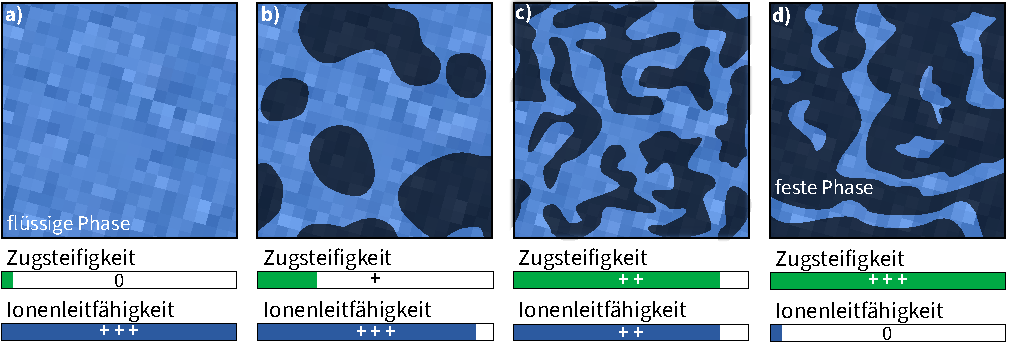
\includegraphics[width=\textwidth, angle=0]{bicontinous_electrolyte.pdf}
		\caption{\label{fig:electrolyte_data}Multifunktionale Performanz von verschiedenen Strukturelektrolyten~\cite{Greenhalgh2023}.}
\end{figure}
Diese Limitierungen schließen die in konventionellen Batterien etablierten flüssigen Elektrolytsysteme kategorisch aus. Gleiches gilt auch für Gelelektrolyte, deren hohe Ionenleitfähigkeit mit sehr geringen mechanischen Eigenschaften einhergeht~\cite{Gayet2009, Li2018, Zhao2020a}. Für den Einsatz in Strukturbatterien kommen daher nur zweiphasige oder feste Elektrolytsysteme in Frage~\cite{Greenhalgh2023}.

%\subsubsection{Zweiphasige Electrolytesysteme}
\begin{figure}[ht]
	%\raggedleft
		%\def\svgwidth{\columnwidth}
        \center
	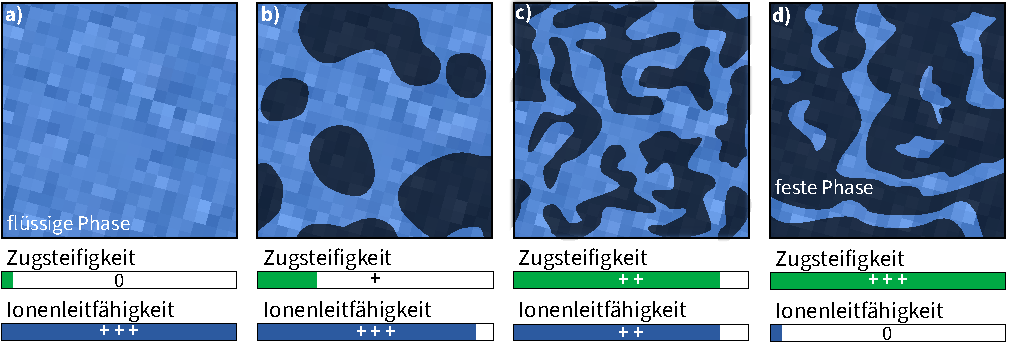
\includegraphics[width=\textwidth, angle=0]{bicontinous_electrolyte.pdf}
		\caption{\label{fig:bicontinous_electrolyte}Veränderung der Zugsteifigkeit und der Ionenleitfähigkeit mit zunehmenden festem Phasenanteil bei zweiphasigen Elektrolyten (a-d).}
\end{figure}
ZZweiphasige Elektrolyte bestehen aus einer festen Phase, die für die mechanischen Eigenschaften verantwortlich ist, und einer flüssigen oder gelförmigen Phase, die für die Leitung der Ionen zuständig ist~\cite{Ichino1995}. Durch die Einstellung des Phasenanteils und die Kontrolle der Porenarchitektur können die resultierenden Eigenschaften zwischen maximaler Leitfähigkeit und minimalen mechanischen Eigenschaften und umgekehrt eingestellt werden, siehe Bild~\ref{fig:bicontinous_electrolyte}. In simulativen Studien wurden mögliche ideale Architekturen und Phasenanteile zur maximalen Steigerung der Multifunktionalität bereits bestimmt~\cite{Lee2019,Tu2020}. Jedoch gibt es bisher nur eine bekannte Studie, die diese Nanostrukturen mithilfe von 3D-Druck fertigte~\cite{Zekoll2018}, die jedoch mit $2,7 \times 10^4$ $\si{\milli \siemens \per \cm}$ den angestrebten Grenzwert nicht überschreiten konnte. Der existierende Stand der Technik konzentriert sich daher hauptsächlich auf die Fertigung relativ ungeordneter Strukturen. Bei der Wahl des Phasenanteils sind dabei auch Untersuchungen aus der Perkolationstheorie, die sich mit der Bildung von weitreichenden Verbindungen in zufälligen Systemen beschäftigt, zu beachten. Untersuchungen mit zufällig angeordneten Kugeln zeigen, dass erst bei einem Anteil von 29,02~\% an leitender Phase ein Grenzwert überschritten wird, bei dem eine durchgehende Verbindung und damit die Möglichkeit des Ionentransports von einer Elektrode zur anderen sichergestellt werden kann~\cite{Li2020b}. Die gleiche Studie zeigt auch, dass durch Abweichung von der sphärischen Struktur dieser Anteil auf 22,94~\% reduziert werden kann. Die Perkolationstheorie ist somit ein wichtiges Mittel zur Untersuchung des Verhaltens von zweiphasigen Elektrolyten und bietet zum Beispiel Erklärungsansätze, warum bei bestimmten Anteilen von flüssiger Phase scheinbar plötzlich eine Steigerung der Ionenleitfähigkeit um mehrere Größenordnungen beobachtet wird~\cite{Melodia2023}.

Für die feste Phase haben sich auf Harz basierte Systeme hauptsächlich wegen ihrer einfacheren Löslichkeit und damit kleineren Porenbildung durchgesetzt. Jedoch treten vermehrt thermoplastische Systeme in den Vordergrund. Diese sind leichter in den Fertigungsprozess zu integrieren und bieten zusätzliche Sicherheit bei auftretenden Kurzschlüssen, da bei der entstehenden Wärmeentwicklung der Thermoplast schmilzt und die Poren verschließt, was einen weiteren Ladungsaustausch unterbindet.

Als Ausgangsmaterialien für die flüssige Phase kommen ionische Flüssigkeiten~\cite{Huang2022,Shirshova2013,Wendong2021,Shirshova2014,Dzienia2020}, Lithiumsalzlösungen in organischen Lösemitteln~\cite{Gienger2015,Sakakibara2017}, deren Kombination~\cite{Shirshova2014,Yu2016} und andere Systeme~\cite{Feng2017} in Betracht.

Feststoffelektrolyten bestehen meist aus einer Polymermatrix mit flexiblen Ketten, um die Bewegung eines gelösten Salzes zu ermöglichen. Der Hauptvorteil dieses Ansatzes liegt im Verzicht auf flüchtige oder brennbare Bestandteile und in den durch das Polymer bestimmten vergleichsweise guten mechanischen Eigenschaften. Allerdings ist die ionische Leitfähigkeit bei Raumtemperatur deutlich geringer als bei zweiphasigen Vertretern. Die Herstellung von Feststoffelektrolyten kann auf zwei Wegen erfolgen. Eine Möglichkeit stellt dabei die Polymerisation in Anwesenheit von Lithiumsalz dar. \textsc{Snyder et al.}~\cite{Snyder2007, Snyder2009} erreichten mit diesem Ansatz Ionenleitfähigkeiten von $1,6 \times 10^{-5}$ - $1,7 \times 10^{-3}$ $\si{\milli \siemens \per \cm}$ und damit verbundene Zugmodule von 552 bis 15~$\si{\MPa}$. Der zweite, häufig verwendete Ansatz nutzt eine Mischung von Polymeren mit Lithiumsalz. Für diese komplett festen zweiphasigen Elektrolytsysteme kommen häufig Epoxid~\cite{Matsumoto2011,Munoz2021,Wang2020b} oder PEO~\cite{Moreno2011,Ji2010,Guo2021} zum Einsatz.

\subsection{Separator}

Separatoren befinden sich zwischen den beiden Elektroden und dienen hauptsächlich dem Verhindern eines elektrischen Kurzschlusses. Daraus folgt die Anforderung, dass Separatormaterialien für Elektronen nicht durchlässig sind, aber Transportmechanismen für Ladungsträger bereitstellen~\cite{Kurzweil2015}. Um Kurzschlüsse auch bei mechanischen Belastungen zu verhindern, werden außerdem Anforderungen an die mechanische Belastbarkeit gestellt~\cite{Asp2015}. Weitere wichtige Eigenschaften sind eine hohe chemische und thermische Stabilität, insbesondere gegenüber Korrosion, geringe Dichte, geringe Dicke, große Verfügbarkeit und damit verbundene geringe Materialkosten~\cite{Beard2019}. Im Kontext von Strukturbatterien und der häufigen Verwendung von festen Elektrolytsystemen ist der Einsatz von Separatoren theoretisch nicht notwendig, da im Gegensatz zu flüssigen Elektrolyten das Auseinanderhalten der Elektroden auch unter Druck gewährleistet werden kann. Jedoch ist im Rahmen von Sicherheitsbedenken und aufgrund einer signifikanten Erschwerung des Herstellungsprozesses ohne diese der Einsatz von Separatoren immer noch ein wichtiges Element in der Konzeptionierung von Strukturbatterien~\cite{Asp2015, Hubert2022}. Das am meisten verwendete Separatormaterial ist Glasfaser~\cite{Zhou2022}. Jedoch existieren auch vielversprechende Kandidaten, wie polymerbasierte Separatoren, Keramiken und Cellulose~\cite{Simon2008, Greenhalgh2023}, siehe Tabelle~\ref{tab:separator_comp}.

\begin{table}[h!]
    \caption{Properties of different types of separators}
    \label{tab_separator_comp}
    %\begin{adjustwidth}{-\extralength}{0cm}
    \newcolumntype{C}[1]{>{\hsize=#1\hsize\centering\arraybackslash}X}%
    \begin{tabularx}{\textwidth}{
    %C{0.6}
    C{1} 
    C{1.8} 
    C{0.8} 
    C{0.8} 
    C{0.8} 
    C{0.6}
    }
        \toprule
        \textbf{Separatortyp}
        &\textbf{Separatormaterial} 
        &\textbf{Ionische Leit- fähigkeit\textsuperscript{*} (mS/cm)} 
        &\textbf{Zug- steifigkeit\textsuperscript{*} (GPa)}
        & \textbf{Festigkeit\textsuperscript{*} (MPa)}
        &\textbf{Ref.} \\
        \midrule
        %\legendsep{c0}&
        Glassfaser&Glassfaser&1.13&21
        &325
        &\cite{Deka2017}\\
        %\midrule
        \addlinespace
        %\legendsep{c10}&
        Polymer&RF/PLA&110&0.3271
        &15.2
        &\cite{Vargun2020}\\
        %\midrule
        \addlinespace
        %Gel polymer electrolyte&$\mathrm{PVA/KOH/K_3[Fe(CN)_6]}$&45.56&n.a.&n.a.&\cite{maHighPerformanceSolidstate2014}\\
        %%\midrule
        %\legendsep{c4}&
        Feststoff- elektrolyt&$\mathrm{PEGDGE/TETA/EMIBF_4}$&0.2&26
        &350
        &\cite{Hubert2022, Choi2022}\\
        %\midrule
        \addlinespace
        %\multirowcell{2}{\legendsep{c6}}&
        \multirowcell{2}{Keramik}
            &$\mathrm{PVDF/PPG/LiCl/CaTiO_3}$&n.a.&1.2
            &65
            &\cite{Alvarez‐Sanchez2019}\\
            &$\mathrm{PVB/Al_2O_3NW}$&13.5&n.a.
            &30
            &\cite{Liu2020a}\\
        %\midrule
        \addlinespace
        %Diode-like polymer electrolyte&PVP/PEI/SWCNT&n.a.&n.a.&n.a.&\cite{chowdhurySupercapacitorsElectricalGates2019}\\
        %%\midrule
        %Ceramic&NPs/PTFE/SiC&n.a.&n.a.&1.3&\cite{qinCeramicBasedSeparatorHighTemperature2018,zhaoInorganicCeramicFiber2017}\\
        %%\midrule
        %Tree-leave&Quercus rubra&n.a.&n.a.&n.a.&\cite{chenTrashTreasureFallen2022,wangMechanicalCharacteristicsTypical2010}\\
        %%\midrule
        %Eggshell membrane&Eggshell membrane&3.8&n.a.&6.59&\cite{yuUsingEggshellMembrane2012}\\
        %%\midrule
        %\legendsep{c8}&
        Cellulose&MCC/AMIM-Cl&298.6&5.43
        &71.71
        &\cite{Ahankari2022, Xu2020}\\
        %%\midrule
        %Graphene oxide&Graphene oxide paper&n.a.&n.a.&n.a.&\cite{shulgaSupercapacitorsGrapheneOxide2015,comptonTuningMechanicalProperties2012}\\
        %%\midrule
        %Metal-organic framework&Metal-organic framework&n.a.&n.a.&n.a.&\cite{mengMetalOrganicFrameworks2015,bundschuhMechanicalPropertiesMetalorganic2012}\\
        \bottomrule
    \end{tabularx}
    %\end{adjustwidth}
    \noindent{\footnotesize{\textsuperscript{*} The abbreviation not available (n.a.) is used.}}
\end{table}

Glasfaserseparatoren finden großen Einsatz wegen ihrer hohen mechanischen Belastbarkeit, ihrer sehr hohen thermischen und elektrochemischen Stabilität und relativ geringen Materialkosten~\cite{Luo2015,Asp2019,Asp2021,Liu2022}. Allerdings haben sie im Vergleich zu anderen Materialkandidaten eine signifikant höhere Dicke und benötigen eine hohe Maschenweite, um einen hohen Ionenaustausch zu ermöglichen, siehe Bild~\ref{fig:separator_transportation}, was allerdings mit einem höheren Kurzschlussrisiko einhergeht~\cite{Danzi2021,Zhou2022}. 

Im Kontext von faserbasierten Separatoren wurden außer Glasfasern auch Aramidfasern eingehend betrachtet~\cite{Jin2023}. Hervorzuheben ist hierbei ihre Fähigkeit, Dendritwachstum zu verhindern, was bei Lithiumionenbatterien oft zu einem besseren Zyklenverhalten gegenüber Glasfasern führt~\cite{Tung2015,Wang2021a}.

\begin{figure}[ht]
	%\raggedleft
		%\def\svgwidth{\columnwidth}
        \center
	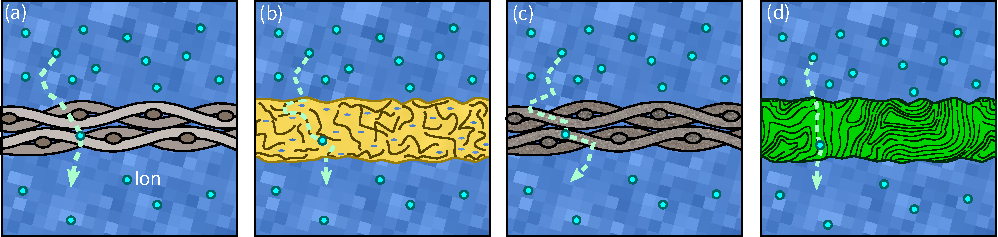
\includegraphics[width=\textwidth, angle=0]{separator_transportation.pdf}
		\caption{\label{fig:separator_transportation}Visualisierung verschiedener Separatormaterialien und der jeweligen Ionentransportwege (gestrichelte Linie) für: (a) Gewebe, (b) Polymer-, (c) Keramikseparator und (d) Cellulose~\cite{Zschiebsch2024}.}
\end{figure}


Materialien für Polymerseparatoren sind oft identisch zu polymerbasierten Festelektrolyten. Bei zweiphasigen Elektrolyten ist besonders die gute Durchdringung des Elektrolyten von Vorteil, die eine um den Faktor 100 höhere Ionenleitfähigkeit als Glasfaserseparatoren ermöglicht~\cite{Wang2021a}. Jedoch führt auch hier die höhere Porosität zu einer Reduktion der mechanischen Eigenschaften und stellt somit einen Zielkonflikt dar~\cite{Ahankari2022}. Dies wird auch in einer Studie von \textsc{Karabelli et al.}~\cite{Karabelli2011} deutlich, bei der die entwickelte Polymermembran eine Zugsteifigkeit von 741~$\si{\MPa}$ erreichte. Im Vergleich reduzierte sich dieser Wert für das gleiche Ausgangsmaterial mit einer Porosität von 75~\% auf 53~$\si{\MPa}$. Im Vergleich zu Glasfaser sind die mechanischen Eigenschaften jedoch signifikant geringer, weshalb Polymerseparatoren außerhalb von flexiblen Anwendungen aktuell keine Rolle spielen~\cite{Zschiebsch2024}.

Keramische Separatormaterialien zeichnen sich besonders durch ihre hohe thermische Stabilität aus und werden daher auch bereits in Batterien mit hohen Betriebstemperaturen eingesetzt~\cite{Qin2017,Cheong2012}. Außerdem bieten diese neben ausgezeichneten thermischen auch hervorragende physikalische und elektrochemische Eigenschaften. Jedoch besitzen derzeit verfügbare keramische Separatoren im Vergleich zu Glasfaser nur eine unzureichende Zugfestigkeit~\cite{Qin2017}. Ein diesbezüglich vielversprechender Entwicklungsansatz ist dabei die Integration von keramischen Fasern, die sowohl als Separatoren als auch zur Verstärkung der Elektrolyt-Matrix dienen. \textsc{Zhao et al.}~\cite{Zhao2017} entwickelten einen keramischen Faserseparator für Lithium-Ionen-Batterien, indem sie unregelmäßige keramische Kurzfasern in die Matrix integrierten. Durch die Konsolidierung der Matrixmaterialien mit kontinuierlichen keramischen Fasern konnte die Festigkeit des Verbundmaterials verbessert werden. SiC-basierte Fasern weisen beispielsweise Zugfestigkeiten von bis zu 6~$\si{\GPa}$ und Elastizitätsmodulwerte von bis zu 420~$\si{\GPa}$ auf~\cite{Seydibeyoglu2017}. Zudem entwickelten \textsc{Yamamoto et al.}~\cite{Yamamoto2009} eine Methode, um ausgerichtete Kohlenstoffnanoröhren auf keramischen Fasern wachsen zu lassen, was die Bindung zwischen Faser und Matrix weiter verstärken und das Porenvolumen des keramischen Faserseparators erhöhen könnte, um die Ionenleitfähigkeit zu verbessern.

Das Interesse an Cellulose ist in den letzten Jahren zusammen mit einem wachsenden Forschungsfeld zu den Themen ''nachwachsende Rohstoffe'' und ''recyclebare elektrische Speicher'' immer mehr gewachsen~\cite{Liang2018,Teng2020}. Cellulose zeigt dabei eine sehr hohe Ionenleitfähigkeit und eine gute, wenn auch im Vergleich zu Glasfasern deutlich geringere, mechanische Festigkeit und Zugsteifigkeit~\cite{Xu2020}, siehe Tabelle~\ref{tab:separator_comp}. Eine Möglichkeit zur Steigerung der Steifigkeit stellt dabei die Verwendung von Nanocellulose dar, die Zugsteifigkeiten von bis zu 130~$\si{\GPa}$ erreicht~\cite{Dufresne2013,Zhang2019}.

\subsection{Pouchfolie}
Herkömmliche Pouchzellen sind mit einer kunststoffbeschichteten Aluminiumhülle vor Umwelteinflüssen geschützt. Insbesondere verhindert diese, dass Feuchtigkeit in die Batterie eindringt und giftige oder brennbare Stoffe aus der Batterie entweichen können. Außerdem ermöglichen die guten mechanischen und Wärmeleiteigenschaften der Aluminiumfolie eine geringe Gesamtmasse und eine effizientere Temperaturregulierung der Zellen. Eine zunehmend wichtiger werdende Aufgabe, die allerdings noch nicht hinreichend erfüllt wird, ist das Aufbringen eines äußeren Zelldrucks.

In mehreren Studien konnte gezeigt werden, dass durch einen hohen externen Druck die Kontaktierung zwischen Elektrode und Elektrolyt verbessert wird, was einen besseren Ionen- und Elektronentransport bewirkt. Außerdem können unerwünschte Nebenreaktionen unterdrückt werden, wie etwa Gasbildung und Dendritwachstum, was den Lithiumverlust beim Laden und Entladen reduziert und somit dem Kapazitätsverlust entgegenwirkt und das Batterieleben verlängert \cite{Mussa2018,Mueller2019,Sakamoto2019}. Besonders Batterien mit Feststoffelektrolyten benötigen einen deutlich höheren Druck, um den Kontakt zwischen Elektrode und Elektrolyt zu gewährleisten \cite{Boaretto2021}. Jedoch existiert zurzeit noch keine zufriedenstellende Lösung. Zwar wird bereits bei der Herstellung mittels Verpressen der Elektroden ein gewisser Druck realisiert, allerdings können größere Drücke damit nicht appliziert oder über längere Zeit aufrechterhalten werden \cite{Garayt2023}. Daher wird oft versucht, durch eine externe Einspannung auf Systemebene diesen Druck aufzubringen. Jedoch entsteht durch die innere Reibung der Batterien kein gleichmäßiger Druckverlauf, was dazu führt, dass äußere Zellen stärker belastet werden und weiter innen liegende Zellen kaum von dem äußeren Druck profitieren. Auch haben höhere Ausgleichsdrücke das Problem, dass diese eine höhere Anstrengung für das Gesamtpaket darstellen, was zu dickeren Materialien und damit einer niedrigeren Gesamtenergiedichte führt.

Einzig die Knopfzellen, die durch eine integrierte Feder einen definierten Druck auf eine im Verhältnis zur Pouchzelle deutlich kleinere Fläche ausüben, sind die einzige bekannte Lösung zu diesem Problem. Hinzukommt, dass auch hier der Massenanteil von Gehäuse zu Zelle deutlich höher ist als bei Pouchzellen.

Für Strukturbatterien sind bisher keine Alternativen zur herkömmlichen Aluminiumpouchfolie untersucht worden \cite{Ye2024}. Jedoch gibt es viele Gruppen, die ihre Strukturbatterien mit Pouchfolie zusätzlich in einen kohlefaserverstärkten Kunststoff einbetten \cite{Pattarakunnan2020,Asp2021}.

\section{Aktuelle Ansätze zur Entwicklung und Auslegung von Strukturbatterien}
Die Variation an verschiedenen Strukturbatterien hat in den letzten Jahren abgenommen~\cite{Asp2024}. In aktuellen Forschungsarbeiten konzentriert sich die Forschungsgemeinschaft hauptsächlich auf verschiedene Kohlefasern als Anode, \ce{FePO4} als Aktivmaterial für die Kathode, eine Vielzahl an verschiedenen zweiphasigen Strukturelektrolyten, Glasfasern als Separatorschicht und konventionellen Pouchfolien~\cite{Asp2021,Jin2023, Asp2024,Chaudhary2024}. Bei den Kohlefasern zielt die aktuelle Forschung darauf ab, die Eigenschaften über die Herstellung zielgerichtet auf die Anforderungen der Strukturbatterie einzustellen~\cite{Asp2024}. Zusammen mit Institutionen wie Carbon Nexus wird dabei versucht, die Mechanismen besser zu verstehen, um die Lithiumdiffusion in die Faser zu beschleunigen, ohne dabei die Faserstabilität zu reduzieren~\cite{Duan2021,Larsson2023,Johansen2024,Asp2024}. Forschungsgruppen wie \textsc{Asp et al.} setzen auf \ce{FePO4} als Kathodenmaterial wegen seiner höheren elektrochemischen Stabilität und leichteren Verarbeitbarkeit~\cite{Asp2021, Siraj2023, Ye2024, Chaudhary2024}. Auch spielt bei deiser Entscheidung die Vergleichbarkeit eine wichtige Rolle, die für die Verbesserung der Kohlefasern notwendig ist und mit einem Wechsel auf z.B. \ce{NMC} nicht mehr gegeben wäre~\cite{Asp2024}. Die aktuellen Strukturelektrolyte sind aus mechanischer Sicht das schwächste Element~\cite{Lee2019,Jin2023}. Die Kombination aus fester Polymermatrix und flüssigem Transportmedium für die Ionen wird allgemein als der vielversprechendste Ansatz betrachtet~\cite{Lee2019,Asp2021, Greenhalgh2023}. Dabei spielt besonders die Kontrolle über die Porenstruktur eine wichtige Rolle~\cite{Lee2019}. Der Einsatz von Glasfasern als Separator und konventionellen Pouchfolien hängt mit der Abkehr von faserbasierten Aufbauten hin zu einem laminatbasierten Design zusammen~\cite{Zhao2020,Xu2022}.

Die ursprüngliche Idee, bei der jede Faser eine zylinderförmige Zelle ist, wurde besonders zu Beginn als vielversprechendes Ziel angesehen~\cite{Ekstedt2010, Leijonmarck2013, Asp2014}. Die gewonnenen Erkenntnisse zeigen jedoch eine Vielzahl an Problemen, wie komplexe Herstellung, hohes Ausfallrisiko und mangelnde strukturelle Performance auf~\cite{Asp2015,Johannisson2018,Asp2021, Ye2024}. Der laminare Aufbau aus mehreren aufeinander liegenden Schichten orientiert sich an dem bereits viel untersuchten Pouchzelldesign und erlaubt somit eine einfachere Herstellung~\cite{Johannisson2018, Xu2022, Siraj2023}. Darüber hinaus ermöglicht die vergleichsweise einfache Integration von gewebten Kohlefaserstrukturen mit signifikant höheren mechanischen Eigenschaften in alle Richtungen~\cite{Xu2022}. Des Weiteren kann durch die Einbringung von Glasfaserseparatoren das Kurzschlussrisiko deutlich reduziert werden, was die Ausbeute und Varianz bei der Herstellung entscheidend verbessert~\cite{Siraj2023}. Pouchfolien spielen in den aktuellen Forschungsarbeiten zu Strukturspeichern nur eine untergeordnete Rolle~\cite{Jin2023}. Beim ''1st Structural Composite Showcase'' in London wurde sogar diskutiert, ob diese bei der Betrachtung von Strukturspeichern keine Rolle spielen sollten~\cite{Asp2024}. Aktuelle Veröffentlichungen zu Strukturbatterien rechnen daher den Massenanteil bei den spezifischen Größen heraus~\cite{Danzi2021,Ye2024}. Leichter Zugang zu konventionellen Pouchbag-Systemen, leichte Verarbeitung und geringe Versagensraten führen dazu, dass fast ausschließlich konventionelle Pouchbagsysteme zum Einsatz kommen~\cite{Jin2023,Ye2024}.

Bei der Entwicklung neuer Strukturbatterien baut die Forschungscommunity hauptsächlich auf eigenen Erfahrungswerten auf. Der angegebene Hauptgrund dafür ist der Mangel an Vergleichbarkeit zwischen den einzelnen Arbeiten, welcher auf einen Mangel an standardisierten Charakterisierungsmethoden zurückzuführen ist. Zukünftig sollen hierfür die über die Jahre ausgebauten Simulationsframeworks von \textsc{Carlstedt}~\cite{Carlstedt2022,Carlstedt2022a,Carlstedt2022b} und \textsc{Johansen}~\cite{Larsson2023,Siraj2023,Johansen2024} Abhilfe schaffen. Diese Modelle setzen bei der Meso- bzw. Partikelebene~\cite{Carlstedt2020b,Carlstedt2022a} an und kombinieren bestehende Batteriemodelle von \textsc{Newman}~\cite{Bernardi1985,Pals1995,Pals1995a,Christensen2006,Newman2021} und \textsc{Doyle}~\cite{Doyle1993,Doyle1995} mit klassischer Mechanik. Durch den Fokus auf kleinere Skalen können z.B. Effekte durch Faserausdehnung infolge von Lithiierung berücksichtigt werden~\cite{Carlstedt2019,Carlstedt2020b,Duan2021,Johansen2024}. Jedoch werden dazu eine Vielzahl an teils aufwendig zu bestimmenden Materialgrößen benötigt, und die Simulation größerer Systeme erfordert aufgrund des hohen Detailgrades eine signifikante Menge an Rechenressourcen~\cite{Carlstedt2019,Carlstedt2020b,Carlstedt2022a}. Optimierungen in diesem Bereich sind ein aktueller Fokus: So konnte die Forschungsgruppe um \textsc{Simone} mit ihrer Methode die Anzahl der zu simulierenden Fasern von 20 auf 25.000 Kurzfasern steigern~\cite{Goudarzi2022}. Jedoch benötigte die Simulation trotzdem noch knapp eine Woche auf einem Hochleistungsrechencluster. Hinzu kommt, dass der bisherige Fokus darauf liegt, die bestehenden Modelle in ihrer gesamten Komplexität unter Berücksichtigung aller Interaktionen hinsichtlich ihrer oft nicht-linearen thermisch, mechanisch, elektrochemisch Zusammenhänge zu implementieren~\cite{Carlstedt2019,Carlstedt2020b,Carlstedt2022a,Johansen2024}. Aktuelle Arbeiten zur Bildung von SEI könnten diesbezüglich zur ersten Erweiterung der bestehenden Modelle über das bereits in der Batterieforschung bekannte hinausführen~\cite{Yuecel2024}. Bisherige Forschungen zu diesem Themenkomplex zeigen jedoch große Varianzen, die vermutlich durch verschiedene chemische Interaktionen hervorgerufen werden~\cite{Rollin2023,Yuecel2024}. Eine Erweiterung der multiskaligen Methode um atomistische Betrachtungen, um diese Effekte vorherzusagen, ist jedoch mit der Gefahr verbunden, den Rechenaufwand durch rechenintensive DFT- oder Molekularsimulationen weiter zu erhöhen~\cite{Franco2019,Li2020a,Rollin2023}. Dies führt dazu, dass die aktuelle Forschung primär auf Experimente vertraut und die aus den physikalischen Simulationsmodellen folgenden Materialparameter erst im Nachhinein, z.B. durch Regressionsverfahren, bestimmt werden~\cite{Franco2013, Carlstedt2022, Carlstedt2023}.

\section{Ungelöste Herausforderungen in der Entwicklung von Strukturbatterien}
Bei dem ''1st Structural Composite Showcase'' 2024 in London waren mit etwas über 80 Teilnehmern fast alle relevanten Forscher auf diesem Gebiet vertreten~\cite{Greenhalgh2024}. Aktuell besteht diese überschaubare Forschungsgemeinschaft hauptsächlich aus Fachleuten der Kohlefasertechnologie, namentlich \textsc{Greenhalgh}~\cite{Greenhalgh2023}, \textsc{Asp}~\cite{Asp2019,Asp2021}, \textsc{Zenkert}~\cite{Zenkert2024} etc., Polymerespezialisten, wie etwa \textsc{Bismarck}~\cite{Bismarck2012}, \textsc{Shirshova}~\cite{Shirshova2013} und Nanomaterialexperten, wie z.B. \textsc{Shaffer}~\cite{Senokos2023}. Fachgebietsübergreifende Expertisen gibt es aktuell kaum, obwohl sich dies in Zukunft mit der Etablierung spezieller Masterprogramme ändern könnte. Auch gibt es aktuell nur sehr wenige Experten mit einem Hintergrund in Batteriechemie und -herstellung~\cite{Asp2013US}. Hinzu kommt, dass es außer den Forschungsgruppen um \textsc{Asp} und \textsc{Zenkert} nur wenige gibt, die ganze Strukturbatterien entwickeln und fertigen können. Dies liegt vor allem an den Schwierigkeiten, eine reproduzierbare und skalierbare Fertigung aufzubauen~\cite{Siraj2023}.

Aufgrund der sehr limitierten Fertigungsmöglichkeiten folgen die gebauten Strukturbatterien vor allem den Forschungstrends rund um \textsc{Asp} und \textsc{Zenkert}. Bei beiden liegt der Fokus hauptsächlich auf den mechanischen~\cite{Carlstedt2019a,Asp2021,Duan2021} und aktuatorischen Eigenschaften~\cite{Carlstedt2023}, was eine mögliche Begründung sein könnte, warum seit 2009 die Energiedichte nur von 35~$\si{\watt \hour \per \kg}$~\cite{Liu2009} auf 41~$\si{\watt \hour \per \kg}$~\cite{Siraj2023} gesteigert wurde, während die Zugsteifigkeit von 0,7~$\si{\GPa}$ auf 26~$\si{\GPa}$ anstieg. Eine weitere Ursache könnte allerdings auch in dem zunehmenden Umschwenken von Lithium zu Natrium liegen, welches hauptsächlich durch wachsendes Umweltbewusstsein motiviert ist~\cite{Peters2022}. Jedoch sind die theoretisch erreichbaren Energiedichten von Natrium signifikant geringer~\cite{Kundu2015}. Hinzu kommen Herausforderungen durch die vergleichsweise langsame Diffusion in die Kohlefasern, deren Steigerung durch das Einbringen von Ionentransportwegen wie etwa Poren direkt mit einem signifikanten Verlust der mechanischen Eigenschaften einhergeht. Des Weiteren wurden aus elektrochemischer Sicht vielversprechendere Kandidaten wie NMC bisher zugunsten von \ce{FePO4} kaum untersucht~\cite{Asp2024}. Hauptausschlaggebend ist hierbei die bisher ungelöste Herausforderung, die NMC-Partikel, die in etwa die gleiche Größe wie der Faserdurchmesser haben, effektiv in das Strukturbatteriedesign zu integrieren~\cite{Asp2014}.

Die Einbeziehung von weniger vertrauten Materialien in die eigene Forschung wird dabei auch durch den in Kapitel~\ref{sec:Ermittlungsverfahren} beschriebenen Mangel an standardisierten Tests bestärkt~\cite{Greenhalgh2024a}. Dieser führt dazu, dass viele Forschungsgruppen eher den eigenen Arbeiten vertrauen und darauf aufbauen, während neue externe Erkenntnisse spärlicher mit einbezogen werden~\cite{Greenhalgh2023, Greenhalgh2024a}. Hinzu kommt, dass simulative Tools zwar beständig weiterentwickelt werden, jedoch oft ein oder zwei Ebenen unterhalb der erstmals evaluierbaren Zellebene beginnen und daher von Skalierungsproblemen geplagt sind~\cite{Franco2019,Giessen2020}. Zusätzlich führt ihr höherer Detailgrad zu einer enormen Menge an zu bestimmenden Materialdaten, die oft signifikant von mehreren Parametern wie Temperatur, Ladegeschwindigkeit usw. abhängen~\cite{Duan2021,Carlstedt2022b}, oft nur sehr aufwendig bestimmt werden können und teils lange Simulationszeiten benötigen~\cite{Franco2019,Carlstedt2022}. Dies führt dazu, dass die meisten simulativen Methoden erst im Nachhinein benutzt werden, wo fehlende Daten durch Fitting bestimmt werden können~\cite{Carlstedt2022a, Carlstedt2023}. Damit dienen die aktuellen Simualtionstool primär das Verständnis des jeweiligen Einflusses zu verstehen, aber nicht um die aufwendigen Experimente zu ersetzen~\cite{Franco2013}. Die Herausforderung, den Strukturbatterieentwicklungsprozess durch digitale und datengetriebene Ansätze zu beschleunigen, ist daher bisher ungelöst.

Als Letztes besteht die Herausforderung, die Strukturbatterien in die breite Anwendung zu überführen. Das oft erwähnte Ziel des elektrischen Fliegens ist aufgrund der vielen Regularien eine Anwendung, die erst bei signifikanten Performancevorteilen gegenüber den konventionellen Lösungen überhaupt in Betracht zu ziehen ist.~\cite{Scholz2018,Schaefer2018,Ishfaq2022} Auch für Anwendungen in Autos sind die aktuell zu geringen Energiedichten, Sicherheitsbedenken und Schwierigkeiten, verbunden mit dem Auswechseln dieser hochintegrativen Lösung, ein wesentliches Problem~\cite{Kalnaus2021,Martins2021, Carlstedt2020a}. Eine fundierte Betrachtung und Erörterung potenzieller Anwendungen ist daher von großer Relevanz.

(siehe Abschnitt \ref{ch:anhang})